\documentclass[12pt]{article}
\usepackage{fancyheadings, graphicx}
\setlength{\headsep}{2ex}
%----- exact 1-in margins
% NB: headheight and headsep MUST exist and be set
\setlength{\textwidth}{6.5in}
\setlength{\textheight}{9in}
\addtolength{\textheight}{-1.0\headheight}
\addtolength{\textheight}{-1.0\headsep}
\setlength{\topmargin}{0.0in}
\setlength{\oddsidemargin}{0.0in}
\setlength{\evensidemargin}{0.0in}

%----- typeset certain kinds of words
\newcommand{\observatory}[1]{\textsl{#1}}
\newcommand{\package}[1]{\textsf{#1}}
\newcommand{\project}[1]{\textsl{#1}}
\newcommand{\an}{\package{Astrometry.net}}
\newcommand{\boss}{\project{BOSS}}
\newcommand{\des}{\project{DES}}
\newcommand{\euclid}{\observatory{Euclid}}
\newcommand{\EA}{\observatory{Exoplanet Archive}}
\newcommand{\gaia}{\observatory{Gaia}}
\newcommand{\Gaia}{\gaia}
\newcommand{\galex}{\observatory{GALEX}}
\newcommand{\Kepler}{\observatory{Kepler}}
\newcommand{\kepler}{\Kepler}
\newcommand{\lsst}{\observatory{LSST}}
\newcommand{\MAST}{\observatory{MAST}}
\newcommand{\sdss}{\observatory{SDSS}}
\newcommand{\Spitzer}{\observatory{Spitzer}}
\newcommand{\spitzer}{\Spitzer}
\newcommand{\TESS}{\observatory{TESS}}
\newcommand{\thetractor}{\package{The~Tractor}}
\newcommand{\wfirst}{\observatory{WFIRST}}
\newcommand{\latin}[1]{\textit{#1}}
\newcommand{\eg}{\latin{e.g.}}
\newcommand{\etal}{\latin{et~al.}}
\newcommand{\etc}{\latin{etc.}}
\newcommand{\ie}{\latin{i.e.}}
\newcommand{\vs}{\latin{vs.}}

%----- math shih
\newcommand{\given}{\,|\,}

%----- typeset journals
% \newcommand{\aj}{Astron.\,J.}
% \newcommand{\apj}{Astrophys.\,J.}
% \newcommand{\apjl}{Astrophys.\,J.\,Lett.}
% \newcommand{\apjs}{Astrophys.\,J.\,Supp.\,Ser.}
% \newcommand{\mnras}{Mon.\,Not.\,Roy.\,Ast.\,Soc.}
% \newcommand{\aap}{Astron.\,\&~Astrophys.}

%----- Tighten up paragraphs and lists
\setlength{\parskip}{0.0ex}
\setlength{\parindent}{0.2in}
\renewenvironment{itemize}{\begin{list}{$\bullet$}{%
  \setlength{\topsep}{0.0ex}%
  \setlength{\parsep}{0.0ex}%
  \setlength{\partopsep}{0.0ex}%
  \setlength{\itemsep}{0.0ex}%
  \setlength{\leftmargin}{1.0\parindent}}}{\end{list}}
\newcounter{actr}
\renewenvironment{enumerate}{\begin{list}{\scriptsize{\textbf{\textsf{(\arabic{actr})}}}}{%
  \usecounter{actr}%
  \setlength{\topsep}{0.0ex}%
  \setlength{\parsep}{0.0ex}%
  \setlength{\partopsep}{0.0ex}%
  \setlength{\itemsep}{0.0ex}%
  \setlength{\leftmargin}{1.0\parindent}}}{\end{list}}

%----- mess with paragraph spacing!
\makeatletter
\renewcommand\paragraph{\@startsection{paragraph}{4}{\z@}%
                                    {1ex}%
                                    {-1em}%
                                    {\normalfont\normalsize\bfseries}}
\makeatother

%----- Special Hogg list for references
  \newcommand{\hogglist}{%
    \rightmargin=0in
    \leftmargin=0.25in
    \topsep=0ex
    \partopsep=0pt
    \itemsep=0ex
    \parsep=0pt
    \itemindent=-1.0\leftmargin
    \listparindent=\leftmargin
    \settowidth{\labelsep}{~}
    \usecounter{enumi}
  }

%----- side-to-side figure macro
%------- make numbers add up to 94%
 \newlength{\figurewidth}
 \newlength{\captionwidth}
 \newcommand{\ssfigure}[3]{%
   \setlength{\figurewidth}{#2\textwidth}
   \setlength{\captionwidth}{\textwidth}
   \addtolength{\captionwidth}{-\figurewidth}
   \addtolength{\captionwidth}{-0.02\figurewidth}
   \begin{figure}[htb]%
   \begin{tabular}{cc}%
     \begin{minipage}[c]{\figurewidth}%
       \resizebox{\figurewidth}{!}{\includegraphics{#1}}%
     \end{minipage} &%
     \begin{minipage}[c]{\captionwidth}%
       \textsf{\caption[]{\footnotesize {#3}}}%
     \end{minipage}%
   \end{tabular}%
   \end{figure}}

%----- top-bottom figure macro
 \newlength{\figureheight}
 \setlength{\figureheight}{0.75\textheight}
 \newcommand{\tbfigure}[2]{%
   \begin{figure}[htp]%
   \resizebox{\textwidth}{!}{\includegraphics{#1}}%
   \textsf{\caption[]{\footnotesize {#2}}}%
   \end{figure}}

%----- deal with pdf page-size stupidity
\special{papersize=8.5in,11in}
\setlength{\pdfpageheight}{\paperheight}
\setlength{\pdfpagewidth}{\paperwidth}

% no more bad lines!
\sloppy\sloppypar

  \renewcommand{\headrulewidth}{0pt}
  \pagestyle{fancy}
  \lhead{\textsf{David W. Hogg / New Probabilistic Methods for Observational Cosmology}}
  \rhead{\textsf{\thepage}}
  \cfoot{}

\newcommand{\dd}{\mathrm{d}}
\newcommand{\data}{D}
\newcommand{\intrinsic}{\epsilon}
\newcommand{\shear}{\gamma}
\newcommand{\psf}{\psi}

\begin{document}\sloppy\sloppypar

\paragraph{Introduction}
This proposal is to improve the way we make cosmological measurements.
It is to make this improvement by building and bringing to the
community practical tools for performing probabilistic inference with
cosmological data sets.

The scale of cosmological surveys---in terms of sky area ($\pi$ to
$4\pi$ steradians), number of sources ($10^6$ to $10^9$), dynamic
range (the faintest sources can be 8~mag fainter than the brightest
sources), and heterogeneity of scientific objectives (luminosity
functions, expansion history, baryon acoustic feature)---makes them
inhospitable playgrounds for principled probabilistic inference.
Probabilistic inference (think:\ likelihood function and possibly also
Bayes) requires (in the cosmological context) generating the data, in
the sense of either being able to \emph{simulate} the data (with all
its warts) or else being able to write down a \emph{probability
  distribution in the space of the data}.
In either case, the problem is very hard:
The rawest data (pixel intensities read out by the CCD) are related to
the quantities of greatest interest only extremely indirectly, through
a model that includes not just fundamental cosmology but also the
formation of galaxies within the dark-matter density field, star
formation, intergalactic medium physics, emission and absorption and
distortions from the Earth's atmosphere, and an exceedingly complex
telescope and camera.
(We are not going to solve \emph{all} of these problems in this proposal!)

That is, it is for \emph{very good reasons} that the standard practice
of observational cosmology has a ``traditional'' feel to it:
In a typical large-scale structure survey, the standard practice is to
image the sky, create a catalog of sources, obtaining a best value for
each source's redshift (by spectroscopy or photometric redshift
estimation), compute a standard point estimate of the auto-correlation
function, and then perform cosmological inferences on that correlation
function.
This is a daisy-chain of lossy data-analysis steps; information is
lost (and noise propagation becomes approximate or impossible) each
time an intermediate point-estimate is made.
Any juncture at which we can remove one of these lossy steps, or
replace it with an information-preserving step, we will improve our
inferences, in terms of bias, and sometimes also variance.

This proposal is motivated by four observations:

1. Surveys getting bigger, questions getting more subtle, biases
(systematic errors) more likely to dominate.

...Stage-III and Stage-IV projects...

2. There is a bias--variance trade-off, and the harder your
assumptions, the smaller your variance but the bigger your bias!

3. It costs information to make conclusions about things you don't
care about.

4. Amazing progress has been made, in the PI's group and in the
community, in large, principled inferences.  Much of the credit for
this goes to applied math and computational stats.

...Why doing the right thing would be hard

...Example:  Using p(z) in standard large-scale structure!

...Want to develop more fully the ``theory'' of experimental cosmology

\paragraph{Why this PI?}
...What have we achieved so far?

...In exoplanets

...In weak lensing; \thetractor.

...How are we making these things possible?  Applied-math developments

...Very fast GPs

...Samplers that don't require tuning

...Importance sampling for hierarchical inference

...Aside:  $p(d\given z)$ vs $p(z\given d)$

...Aside:  ABC on cosmological data

...Pedagogical role in the community

\paragraph{\package{Toolset 1}: Density-field inference and marginalization}

...theory paper

...expansion for the correlation function and kernel

...toolset and demo on BOSS data

...ab-initio run on some new data sets; could be XXX

\paragraph{\package{Toolset 2}: Using and improving probabilistic redshift information}

\paragraph{\package{Toolset 3}: Creating and using probabilistic shape and PSF information}

Cosmic shear, small distortion of the images of distant
galaxies by large-scale structure in the universe,
is a major probe of cosmolgy. Measurement of the cosmological
weak lensing signal provides extremely powerful probe of the
evolution of dark energy, since the shear signal depends on
both the growth of structure, and the distance-redshift relation.
In this document we present tractable probabilistic methods that
make less constraining assumption about the flow of information
from the data to the cosmological parameters, and help us fully exploit
the potential of weak lensing in  constraining cosmology using the
imaging data from wide field surveys.

PSF estimation for weak lensing:
Extracting the cosmic shear from galaxy images is one of the most challenging tasks in astronomical
data analysis. Shear signal induced by lensing on the images of background galaxies
is coherent but much smaller than the typical 
ellipticities of those galaxies. Moreover, the image of lensed galaxies is convolved with 
an unknown spatially varying kernel, the Point spread function, whose typical
anisotropy is greater than the cosmic shear itself.
 
Effectively, we have 
noisy estimates of the PSF at the positions of stars. We need to use these estimates to infer the
underlying two dimenstional pattern of the PSF. The spatial variation at large angular scales is 
generally smooth and can be well-modeled by the high signal-to-noise stars. However, both atmospheric
turbulance and telescope optics, introduce PSF that varys on scales smaller than the distance
distance between the bright stars. 

Inaccurate estimation of the PSF at the positions of galaxies will lead to bias in shear estimates,
which will propagate into the dark energy constraints if not accounted for. In order to
tackle this issue, we propose to infer the propability distribution function over the PSF
at the positions of galaxies, so that we can marginalize over the PSF instead of treating it 
as a rigid object.

This probability distribution function (a) needs to be flexible enough to capture the complicated 
features of the shape of the PSF as well as its spatial variation, (b) needs to propagate uncertainties
from the pixel level to the PSF, and (c) needs to be easy to evaluate and easy to sample from. By 
projecting the images of stars into lower dimensional KL basis, and imposing Gaussian Process priors 
over each direction of the KL basis we satisfy all the mentioned requirements. This model successfully propagates
the uncertainties in the form of a posterior PDF over PSFs; 
that is, it returns probabilistic information about the PSF at the positions of galaxies. At each
position of the astronomical image, this posterior PDF has a simple form of a Gaussian.

We also examine the performance of this method on estimation of the PSF for simulations 
of \lsst. First, we identify the bright stars on the image and then we randomly divid
them to training set and validation sets of equal size. After learning the KL basis and 
hyper parameters of the Gaussian Process model in the training set, we infer the posterior 
PDF of PSF at the position of stars in the validation set. Figure [\ref{1}] shows a star
in the validation set, and three different draws from the posterior PDF of PSF at that position.

probabilistic inference of shear:
Typically, after measuring the shapes
of a large ensemble of galaxies in a way that
the effect of PSF is elliminated, ellipticities
of these galaxies are averaged together in order to
find a point estimator of the shear.
The methods based on ensemble averaging make strong assumption
about the probability distribution of the intrinsic shape parameters,
and are able to deliver unbiased estimate of shear only if we
have access to unbiased measurements of individual galaxy
ellipticites. 

Our aim is to deliver a fully probabilistic approach for estimation of shear.
We want to write down a likelihood function $p(\data_n\given\shear)$, where $\{\data_n\}$
represents the set of galaxy images. In order to do so, we need to marginalize over the
nuisance parameters that we do not care about. This set of nuisance paramters includes 
shape parameters (e.g., ellipticities), non-shape parameters (e.g., flux, centroid, etc.)
of galaxies, and also the PSF

\begin{eqnarray}
p(\data_n\given\shear)
  &=& \int p(\data_n\given\intrinsic_n , \omega_{n}, \psf , \shear)
  \,p(\intrinsic_n, \omega_{n})\,p(\psf)\,\dd\intrinsic_n\,\dd\omega_n\,\dd\psf
  \quad ,
\label{integral}
\end{eqnarray}
where $\{\intrinsic\}$ ($\{\omega_{n}\}$) represents the set of shape
(non-shape) parameters.

Schematically, equation (\ref{integral}) can be shown by the probabilistic
graphical model (PGM) in Figure[\ref{2}]. Therefore, in this model we need
a prior PDF over intrinsic (unlensed, PSF deconvolved) parameters of galaxies.
This can be done by (a) finding a deep subset (containing a large number of high
signal-to-noise galaxies) of the data, (b) finding the maximum-likelihood estimates
of parameters of those galaxies, (c) and fitting an empirical prior to those parameters. 

Importance sampling ........

multi-exposure data:
The imaging data from the upcoming WL surveys will consists of several
short exposures of each individual galaxy. Stacking has been widely used
as a method to combine information from multiple exposures. 
Although stacking is able to deliver high signal-to-noise images, it distroys a
huge amount of information regarding the spatial variation of
the PSF, and it involves image transformation that could lead to correlated noise
in the final product and distortion of the PSF.

An important advantage of our model is that it can be easily extended
to making inference of shear from multi-exposure data. The graphical model 
regarding corresponding to application of our probabilistic inference to
multi-exposure data is shown in Figure[\ref{3}].

\paragraph{Prior NSF support}

...Fergus grant

...In addition to this NSF support, NASA support and Moore--Sloan.

...Moore--Sloan \emph{not} providing direct research support!

\paragraph{Broader impacts}

\paragraph{Project management and products}

...Just a PI and students

...Theory papers in year 1

...Tool papers with small demos in year 2

...New large-scale data analyses in year 3

...Open-source toolkits

...Hack Days and Weeks

\paragraph{References cited}

\clearpage

\begin{figure}[!htb]
\minipage{.8\textwidth}
  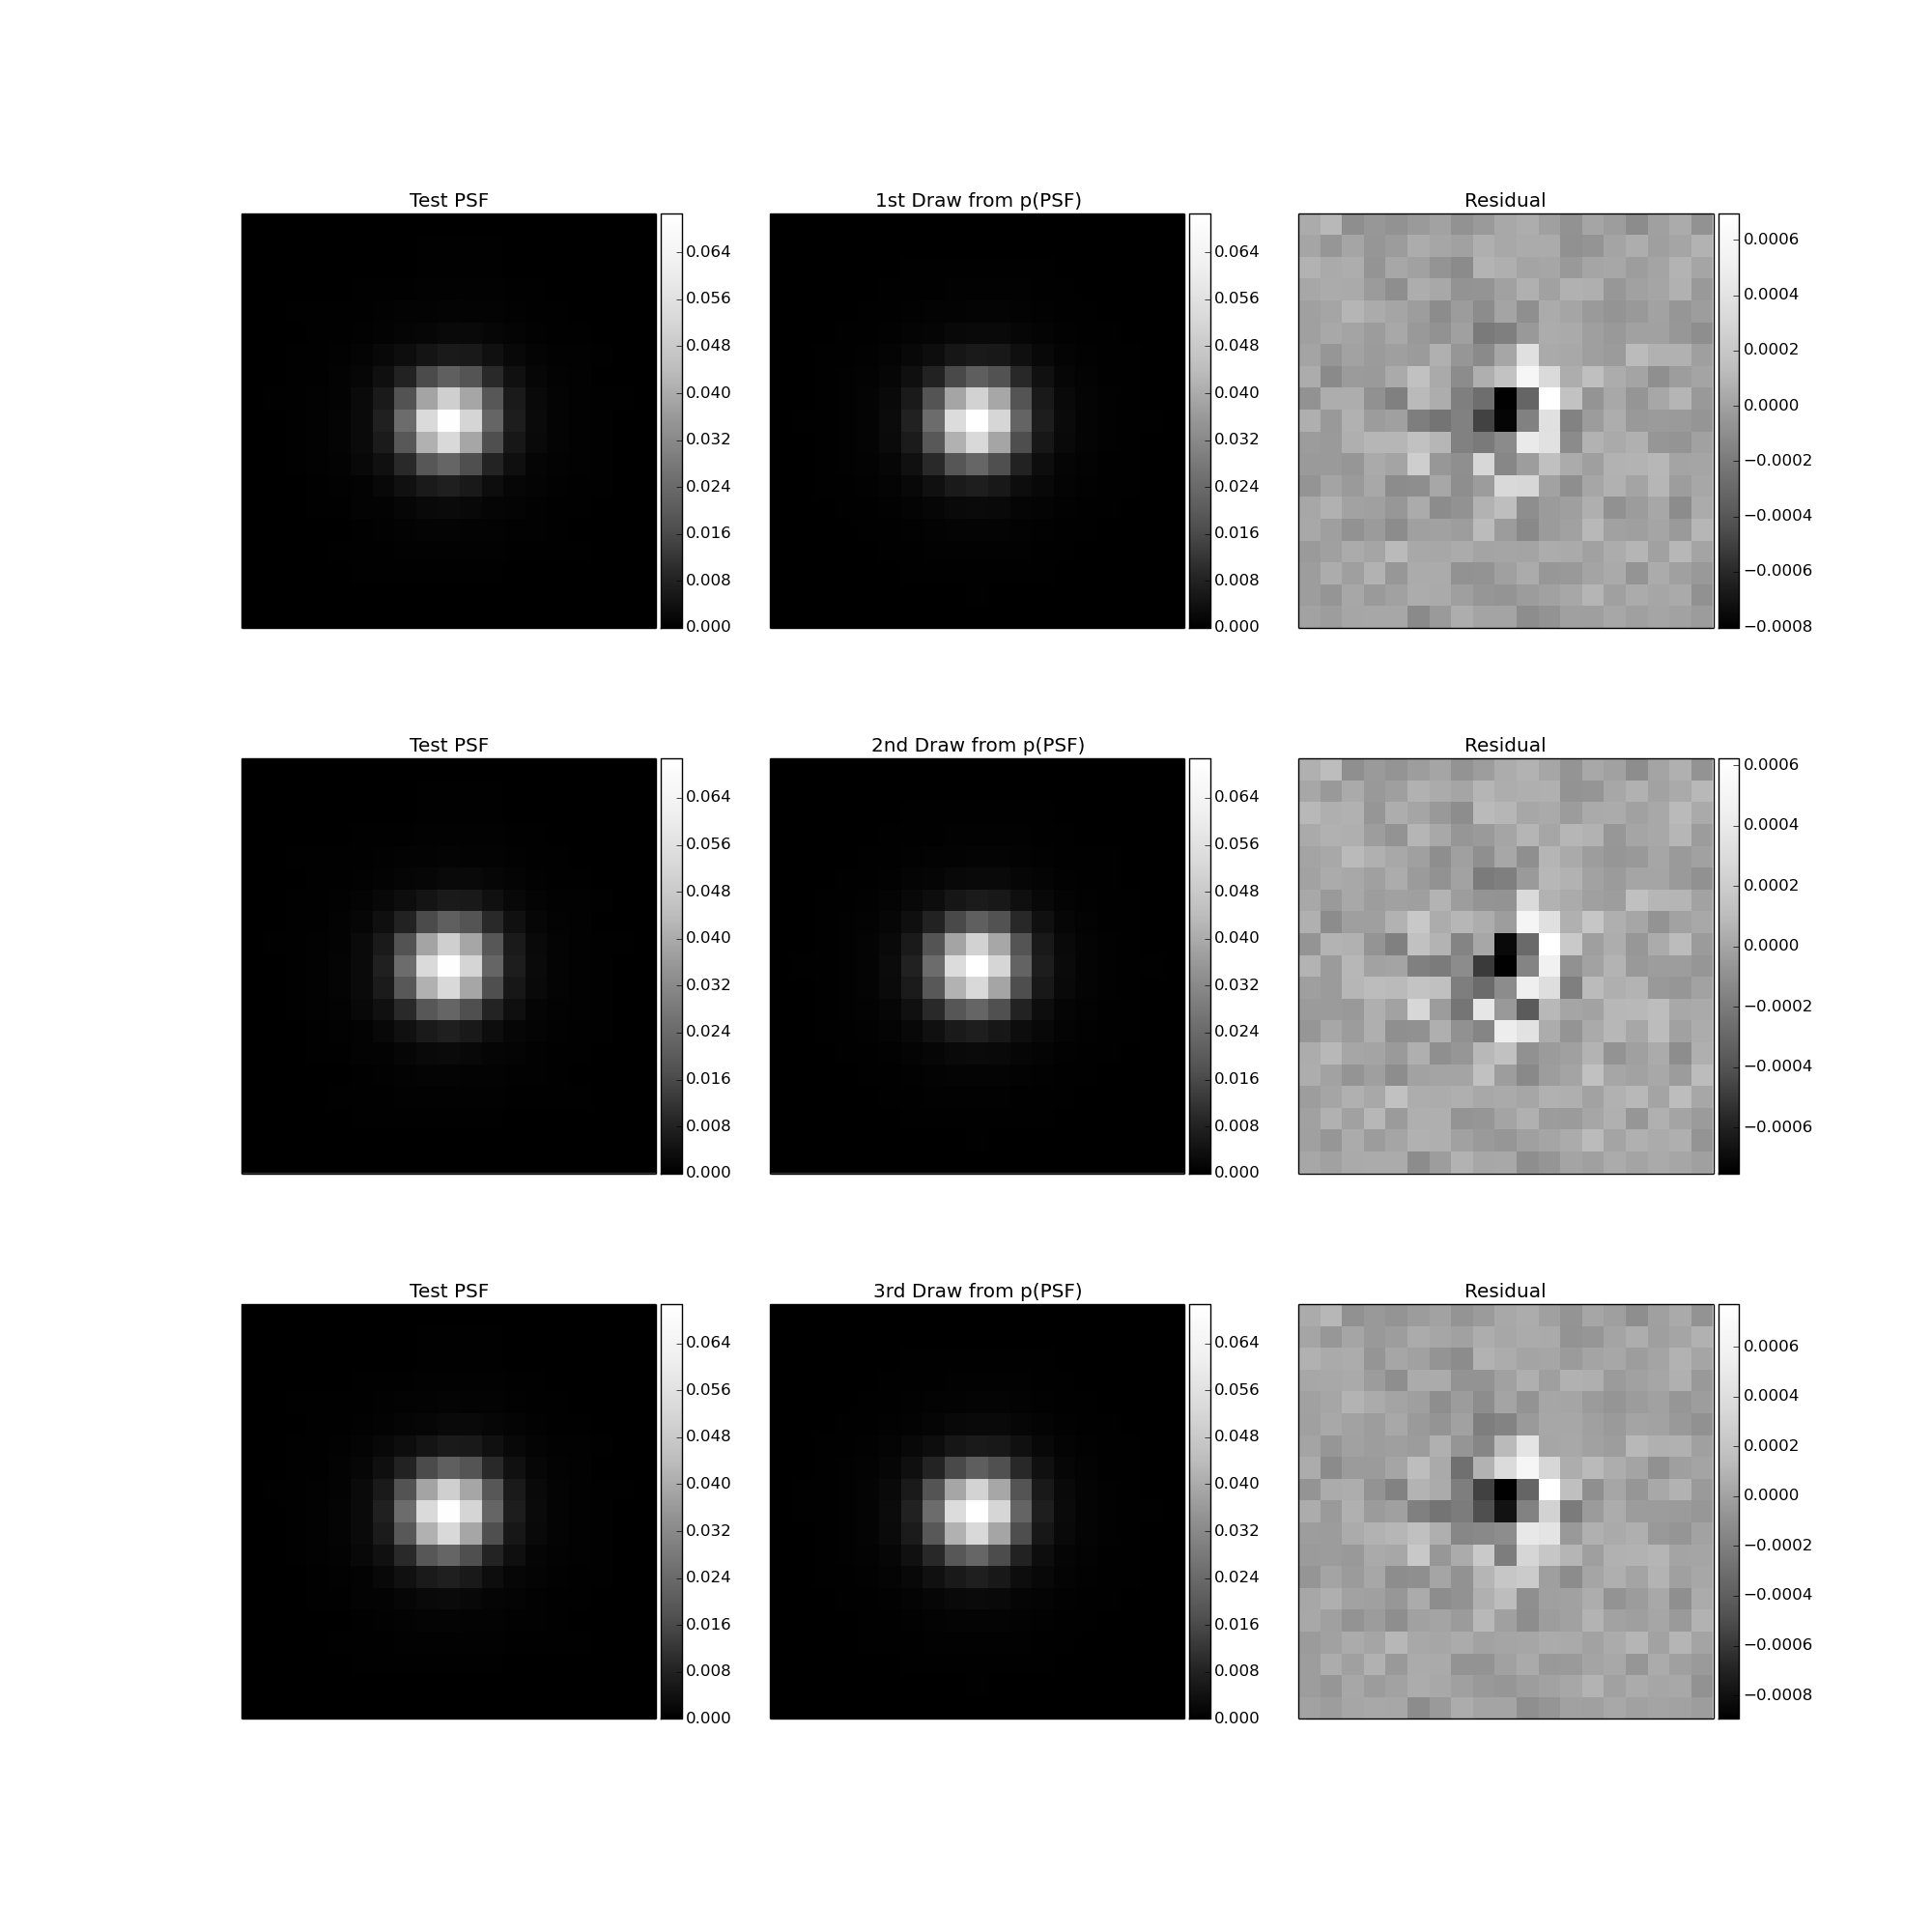
\includegraphics[width=\linewidth]{112.png}
\endminipage
\caption{Plots showing a star in the validation set
(first column), and three different draws (second column)
from our probabilistic PSF model at the
position of star, and the residuals (third column).\label{1}}
\end{figure}

\begin{figure}[!htb]

\minipage{.3\textwidth}
  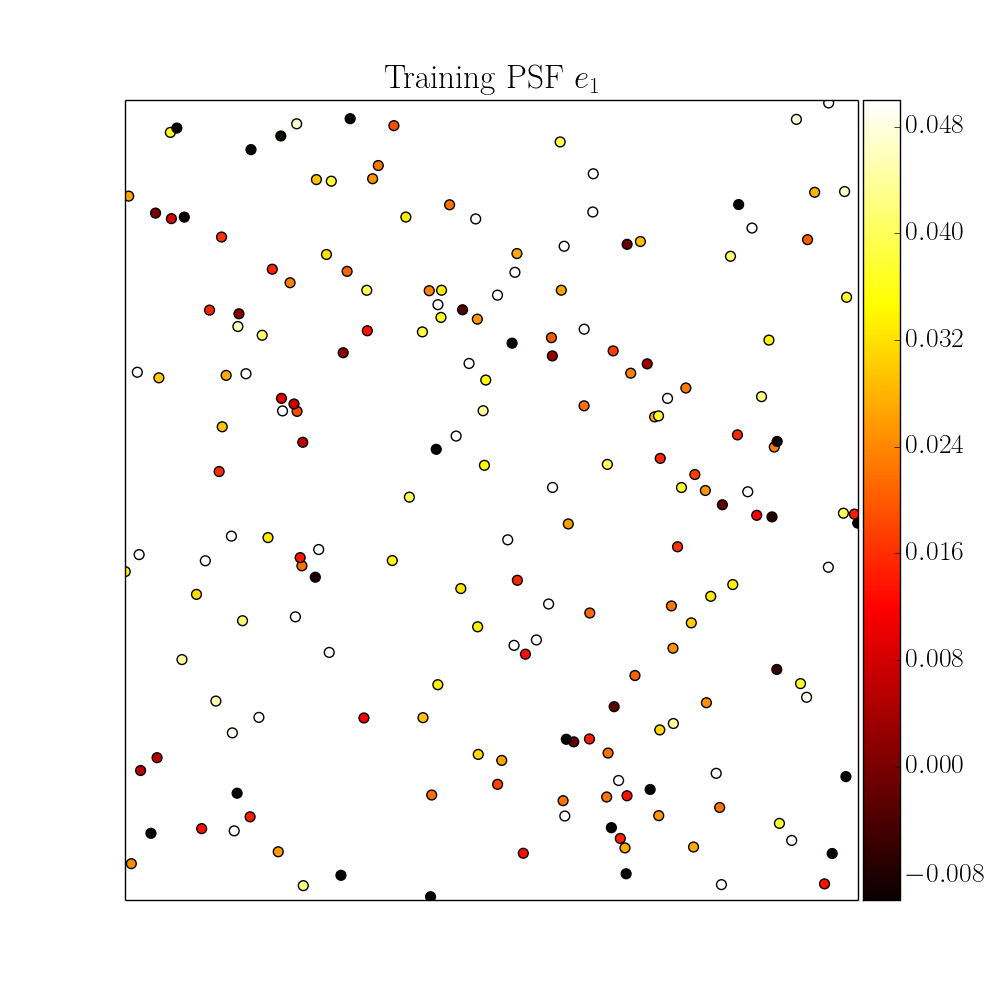
\includegraphics[width=\linewidth]{data_e1.png}
\endminipage

\minipage{1.\textwidth}
  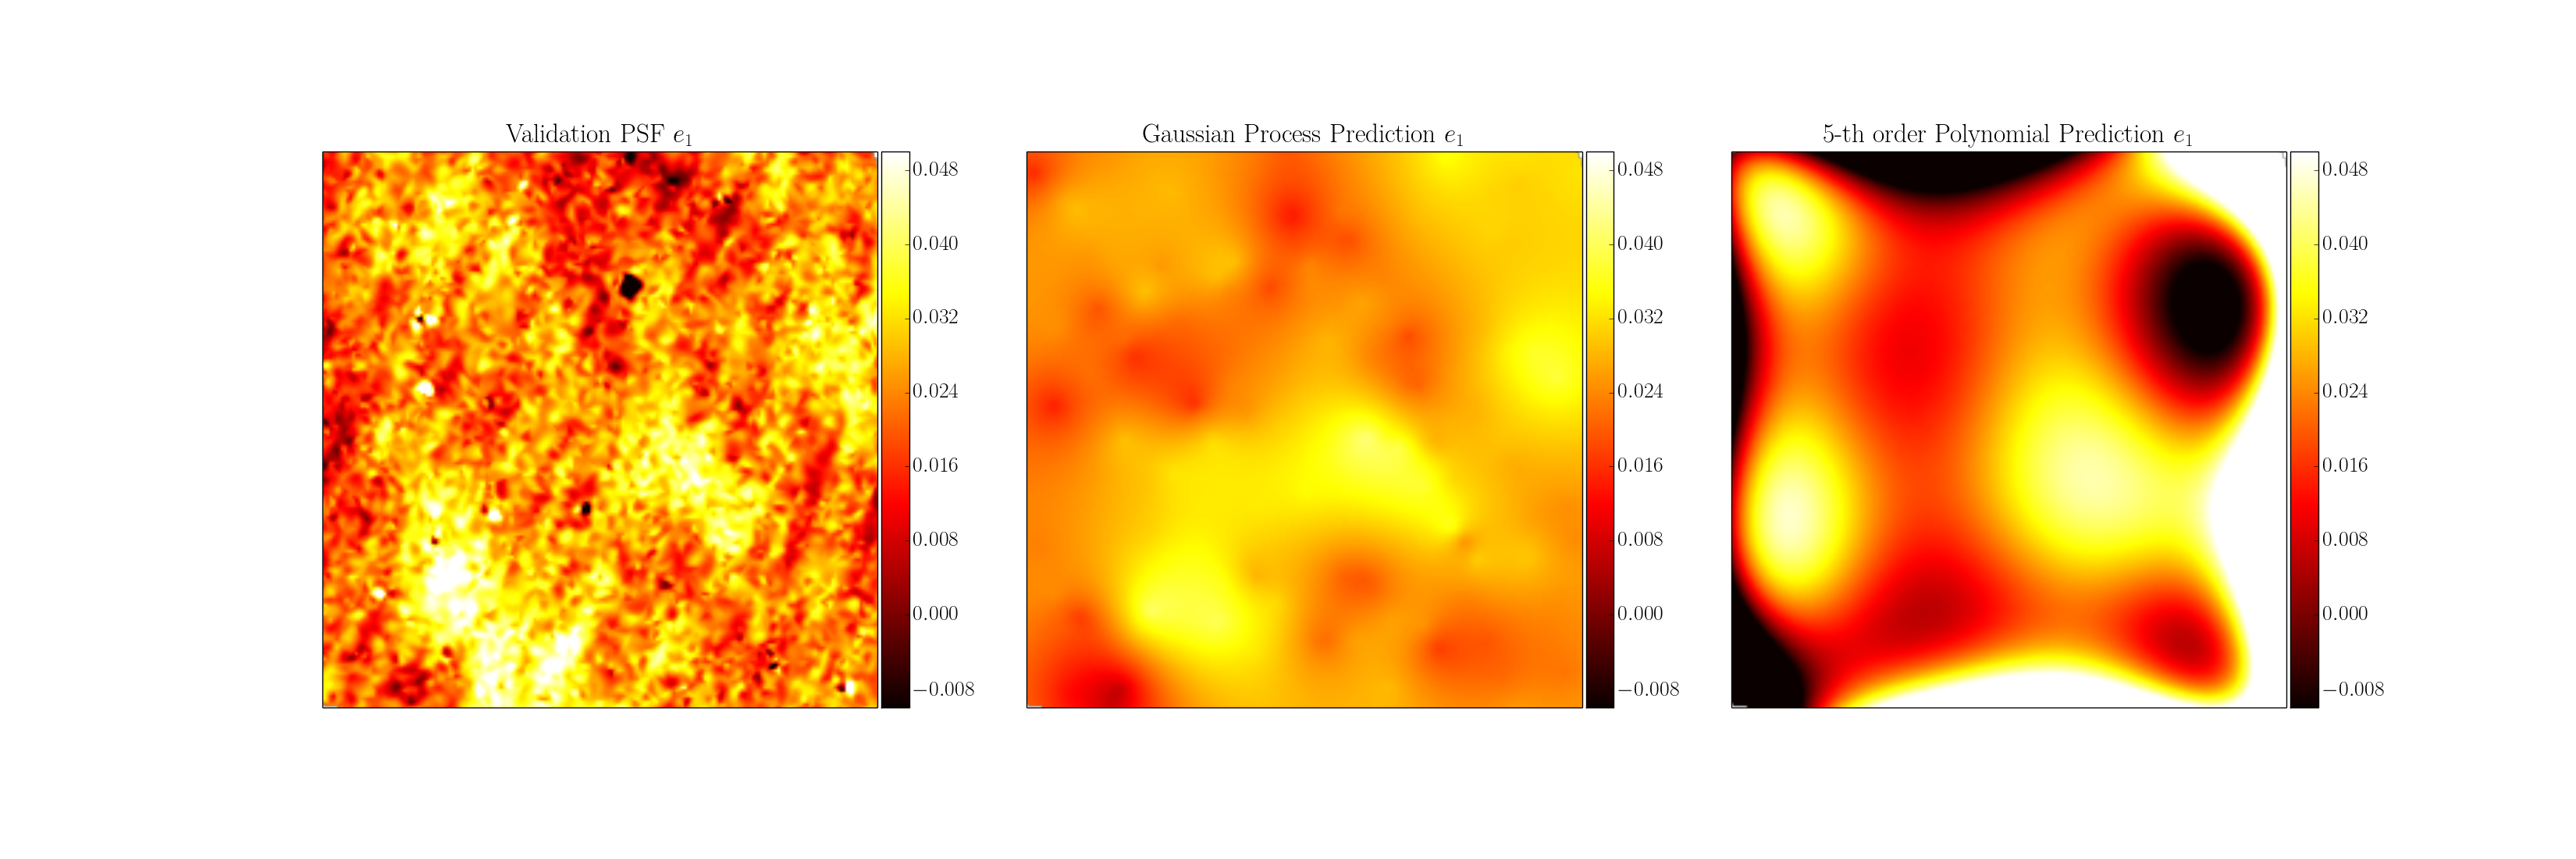
\includegraphics[width=\linewidth]{validation_e1.png}
\endminipage

\caption{Top: scatter plot showing the first components of the ellipticities
of the atmospheric PSF in LSST short exposure imaging data. 
Bottom: Map showing the underlying pattern of atmospheric PSF ellipticities (left),
mean of the posterior probability(middle), and the prediction of 5-th
order polynomial regression (right).
\label{2}}
\end{figure}

\begin{figure}[!htb]
\minipage{.8\textwidth}
  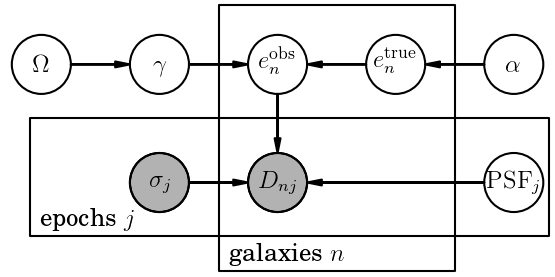
\includegraphics[width=\linewidth]{weaklensing1.png}
\endminipage
\caption{PGM showing the flow of information
from cosmological parameters $\Omega$, PSF at different
exposures $\psf_j$, and 
the underlying distribution of shape parameters 
$\alpha$, to the data at each exposure $\data_{nj}$.\label{3}}
\end{figure}



\end{document}
